%#!pdflatex Naruse_Esurf_2020.tex

Turbidity currents are sediment-laden density flows that occur intermittently in deep sea environments \citep{Talling2014}. Turbidity currents are the main drivers of mass circulation processes in deep sea environments. In fact, estimating the flux of organic carbon transported and buried by turbidity currents is particularly necessary to understand the carbon cycle processes \citep{Buscail1997,Heussner1999}. In addition, the deposits of turbidity currents, i.e., turbidites, form a submarine fans on the sea floor, which may function as large-scale hydrocarbon reservoirs \citep{Kendrick1998,Yoneda2015}, and are thus economically essential.

Through recent development of observational instruments, the velocity and flow depth of deep-sea currents can be measured directly \citep{Clarke2016}. Consequently, numerous records of turbidity currents have been reported at locations such as Squamish Bay, Canada \citep{Clarke2016}, Monterey canyon offshore California \citep{xu2004insitu,xu2010normalized,Paull2018}, and the Congo Submarine Channel \citep{vangriesheim2009turbidity,azpiroz2017newly}. Surprisingly, these records revealed that turbidity currents occurs almost monthly in the modern submarine environments \citep{Paull2018}. On the contrary, the record in Squamish indicated seven events even in one day. However, the turbidites observed in outcrops and cores are deposited at intervals of 500-1000 years or longer. For example, \citet{Ishihara1997} investigated the deposits of the fore-arc basin (the Pliocene Awa Group) and reported that turbidite beds were deposited approximately once every 1200-1300 years. \citet{Clare2014} analyzed turbidites in the western Mediterranean Sea, off the northwest coast of Africa and the Apennines, and found that they were deposited with a frequency of about 1,400-36,000 years in all regions. In contrast to these geologic records, the recent field observations show that turbidity currents are not a rare event.

What caused the difference in observed frequency of modern turbidity currents compared with the records of ancient turbidites? One of the possibilities is that most of the turbidity currents observed in the present day may be very small in magnitude or are diluted, and leave little or no deposits in large areas. If this is the case, turbidites of several tens of centimeters thick observed in geologic records can be interpreted as deposits of extraordinarily large-scale events that occurred once every several hundred years. This hypothesis implies that turbidites in the strata resulted from low-frequency but very high-risk events such as large tsunamis and earthquakes \citep{Goldfinger2003a}. In this case, we would have to assume that the velocity and concentration of turbidity currents obtained from in-situ observations are quite different from those of turbidite-forming currents in strata. Another possibility is that the areas where turbidity currents have been measured experienced very special conditions and that the frequency of turbidity currents will be significantly reduced even in those areas over long time scales. It is very difficult to determine which of these hypotheses is correct at this time because typical hydraulic conditions under which ancient turbidites were deposited have not been well understood. Although the characteristics of turbidity currents in natural environments have been elucidated rapidly through recent \textit{in situ} observations of flow properties \citep{Paull2018}, the flow characteristics of turbidity currents that form actual submarine fans remain unknown.

The inverse analysis of turbidites in strata may fill the gap between the observations of turbidity currents and the geologic field observations of ancient turbidites. The reconstruction of past conditions by inverse analysis has been a major tool in several research fields including sedimentology and geomorphology. For example, several studies have reconstructed the magnitudes of past tsunamis from tsunami deposits \citep{Jaffe2007, Naruse2017, Mitra2020a}, and \citet{Rossano1996} estimated the behavior of pyroclastic flows using inverse analysis. If the hydraulic conditions of turbidity currents, such as velocity and concentration from turbidites can be reconstructed, it should be possible to verify whether turbidite beds in geologic records were deposited from flows of different scales or not by comparing the reconstructed values with the \textit{in situ} observations. 

However, no practical methodology for the inverse analysis of turbidity currents applicable on a field scale has yet been established. Early attempts to obtain hydraulic parameters of turbidity currents were based on the grain-size distribution of turbidites \citep{SCHEIDEGGER1965,vanTassell1981,Bowen1984,Komar1985,Kubo1995} or on sedimentary structures \citep{Harms1960,Walker1965,allen1982sedimentary,Komar1985,allen1991bouma,baas2000duration}. The estimation of hydraulic conditions for turbidity currents based on grain size assumed that the flow is close to the criteria of suspension or the auto-suspension \citep{Komar1985}, but it has been emphasized that this assumption is highly problematic and leads to significantly different results compared with the actual hydraulic conditions for turbidity currents \citep{Hiscott1994}. Although the methods based on sedimentary structures can provide rough estimates of the conditions of a turbidity current, assumptions regarding the thickness of the flow are required \citep{Ohata2017}. 

To obtain reasonable flow characteristics from turbidites, inverse analysis using a numerical model should be performed. \citet{Falcini2009} proposed a method for predicting the hydraulic conditions of turbidity currents from ancient turbidites and applied it to the Laga Formation in the Central Apennines, Italy. Their steady-state model was largely simplified to obtain an analytical solution of the model. However, most of the ancient turbidites are characterized by graded bedding \citep{Bouma1962}, which suggests non-steady waning nature of currents. Therefore, the applicability of this method should be quite limited to non-graded turbidites deposited from long-maintained flows. Conversely, \citet{lesshafft2011towards} applied a direct numerical simulation model for the inversion of turbidite, whose application however to field-scale data is difficult because of the high calculation cost. \citet{Parkinson2017} proposed a method applicable to non-steady field scale flows by using a layer-average model as the forward model, which is potentially applicable to turbidites in outcrops. However, the flow conditions predicted from ancient turbidites were quite unrealistic in their study. They analyzed a turbidite in the Marnoso Arenacea Formation in the Appennine, and gave flow depth of  3950 m or 1.92 mm; both reconstructions are not acceptable as realistic conditions. These extremely large or small estimates may be due to oversimplification in their forward model or failure in the optimization of the input parameters. \citet{Nakao2017} were the first to successfully perform an inverse analysis of turbidites using a general non-steady layer-averaged model. Although their reconstruction of the hydraulic conditions of the turbidity current was reasonable, the computational load of the inverse analysis was high because they used a genetic algorithm for optimization. Thus, they were unable to repeatedly analyze various artificial or field data to test the validity and robustness of their inverse model. In addition, because of the high computational load, modifying their forward model to a more complex one in future would be difficult. These previous attempts suggest that a robust inverse model that can accept a more complex forward model is required to conduct inversion of turbidity currents from turbidites under realistic conditions.

Here, we propose a new methodology using an artificial neural network (NN) for obtaining flow characteristics of turbidity currents from their deposits (Fig. \ref{fig:schematic_diagram_procedures}). NNs are machine learning systems that can be trained to perform very complex functions \citep{HechtNielsen1987}. NNs have been used in a wide range of applications such as classification \citep{Krizhevsky2012} or generative modeling \citep{Sun2018}. In recent years, this method has been widely applied also in the field of earth and planetary sciences \citep{Laloy2018}. Particularly, NNs are a powerful tool for high-dimensional regression of multiple variables with complex distributions \citep{LeCun2015}. In this study, we generate a non-linear regression model to estimate the hydraulic conditions of turbidity currents from the spatial distribution of bed thickness and grain size of turbidites using NN. If the regression is adequate, the NN can be used as an inverse model of turbidity currents. However, there are too few \textit{in situ} measurements of hydraulic conditions of turbidity currents available. Although it is predicted that at least several hundred datasets of hydrological conditions and depositional characteristics are required to train NN, such frequent observation of turbidity currents that occur intermittently on the deep seafloor cannot be expected. Therefore, the method proposed in this study is designed to generate data of deposits from known conditions by numerical calculations of the forward model. In this case, the generation of training data can be completely parallelized, and therefore, any model that incur a high computational load can be implemented as a forward model. 

In this study, we implement a NN-based inverse analysis and examine its effectiveness for turbidites at the field scale. The focus of this study is on rapidly decelerating sedimentary turbidity currents, and normally graded turbidites are considered to be deposited from such decaying flows. This approach was already proved to be effective for the inverse analysis of tsunami deposits \citep{Mitra2020a}. However, the forward model used in their study was based on the assumption of quasi-steady flow, and thus our work is the first time to perform the inverse analysis using a neural network with completely unsteady flow. The success of the inverse analysis for turbidity currents, which exhibit quite different properties from those of tsunamis, would indicate the wide applicability of our inversion framework for event deposits.

\begin{figure}[t]
  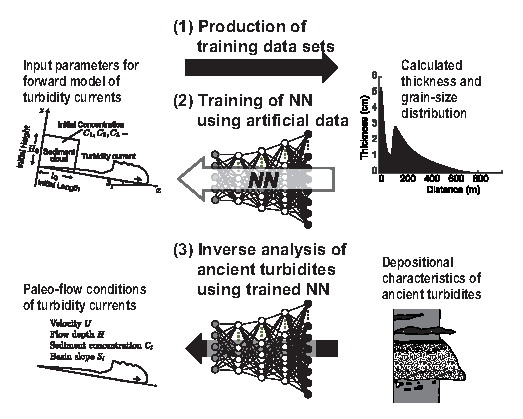
\includegraphics[width=8.3cm]{fig01.eps}
  \caption{Schematic diagram of the inversion process of turbidity currents from deposits. The method is composed of three steps: (1) generation of training data sets by the forward model using random values for model input parameters, (2) trainng of NN based on the artificial data sets, and (3) application of the trained inverse model to unknown field data sets}
  \label{fig:schematic_diagram_procedures}
\end{figure}

